\documentclass[Journal]{article}

%% Please choose the appropriate document class option:
% "Journal" produces double-spaced manuscripts for ASCE journals.
% "NewProceedings" produces single-spaced manuscripts for ASCE conference proceedings.
% "Proceedings" produces older-style single-spaced manuscripts for ASCE conference proceedings. 
%
%% For more details and options, please see the notes in the ascelike-new.cls file.

% Some useful packages...
\usepackage[utf8]{inputenc}
\usepackage[T1]{fontenc}
\usepackage{lmodern}
\usepackage{graphicx}

\usepackage{caption}
\usepackage[style=base,figurename=Fig.,labelfont=bf,labelsep=period]{caption}
\usepackage{subcaption}
\usepackage{amsmath}
%\usepackage{amsfonts}
%\usepackage{amssymb}
%\usepackage{amsbsy}
\usepackage{newtxtext,newtxmath}
\usepackage[colorlinks=true,citecolor=red,linkcolor=black]{hyperref}
%
% Please add the first author's last name here for the footer:
% Note that this is not displayed if the NoPageNumbers option is used
% in the documentclass declaration.
%
\begin{document}
\include{graphicx}
% You will need to make the title all-caps
\title{Introduction to Alderbaran Characteristics and Spectrum}

\author{Zachary Shelton}

\maketitle

% Please include an abstract:
\section{Abstract}
There are billions of stars and celestial bodies that are worthwhile for scientist and astronomers to observe. When focusing on one body, it requires navigating various databases and academic journals to find characteristics of the body. This paper will focus on the star Alderbaran, which is the brightest star in the constellation Taurus. The paper will discuss the characteristics of Alderbaran, including its class, mass, and temperature. It will also outline how to find the same information for other celestial bodies. 

\section{Celestial Databases}
There is so much observational data it feels impossible to find a specific piece of data or information. However, there are tools and databases that can help. The first tool is the \href{https://cds.unistra.fr/}{SIMBAD database}, which is a database of astronomical objects. The database provides basic information about celestial bodies, such as their class, mass, and temperature. There is also second tool is the \href{https://vizier.cds.unistra.fr/viz-bin/VizieR}{VizieR database}, which provides detailed information about similar or same celestial bodies, such as their spectral type, luminosity, and radius. If your interested in exoplanets, there is the Exoplanet Archive, which provides information about observed and theorized exoplanets, such as their mass, radius, and orbital period.

\section{Glossary of Important Terms}
This section will cover a not so comprehensive list of terms used in astronomy and their meanings:
\begin{itemize}
    \item \textbf{Stellar Class} - The class of a star is a letter that represents the temperature of the star. The classes are O, B, A, F, G, K, and M. The O class is the hottest and the M class is the coolest. Astronomers use blackbody radiation and luminosity to determine the temperature of a star.
    \item  \textbf{Blackbody Radiation} - Blackbody radiation is the radiation that is emitted by a blackbody(read more at: \href{https://phys.libretexts.org/Bookshelves/University_Physics/University_Physics_(OpenStax)/University_Physics_III_-_Optics_and_Modern_Physics_(OpenStax)/06%3A_Photons_and_Matter_Waves/6.02%3A_Blackbody_Radiation}{Blackbody Radiation}). By measuring the broad spectrum of wavelengths of stars, scientist to can determine the temperature of the star.
    \item \textbf{Wien's Law} - States the peak wavelength of a blackbody is inversely proportional to the temperature of the blackbody. The law is represented by the equation $\lambda_{\text{max}} = \frac{b}{T}$, where $\lambda_{\text{max}}$ is the peak wavelength, $b=2.89*10^{-3} m \cdot K$ is Wien's constant, and $T$ is the temperature of the blackbody.
    \item \textbf{Stellar Mass} - Astronomers and astorphysicist use the spectrum of the star combined with the star's luminosity to determine the mass of the star. The peak wavelength of a star indicates what a star is made of. 
    \item \textbf{Stellar Luminosity} - A measure of the total energy a celestial body releases each second, this is also know as absolute brigtness. There are many ways to measure this, and there are definite challenges in determining the true brightness of any stellar body far away.(Read More at: \href{https://www.teachastronomy.com/textbook/Properties-of-Stars/Stellar-Luminosity/}{Stellar Luminosity})
\end{itemize}

\section{Alderbaran}
To find the characteristics of Alderbaran, head to the \href{https://simbad.cds.unistra.fr/simbad/}{SINBAD Database}. 
\begin{figure}[H]
    \centering
    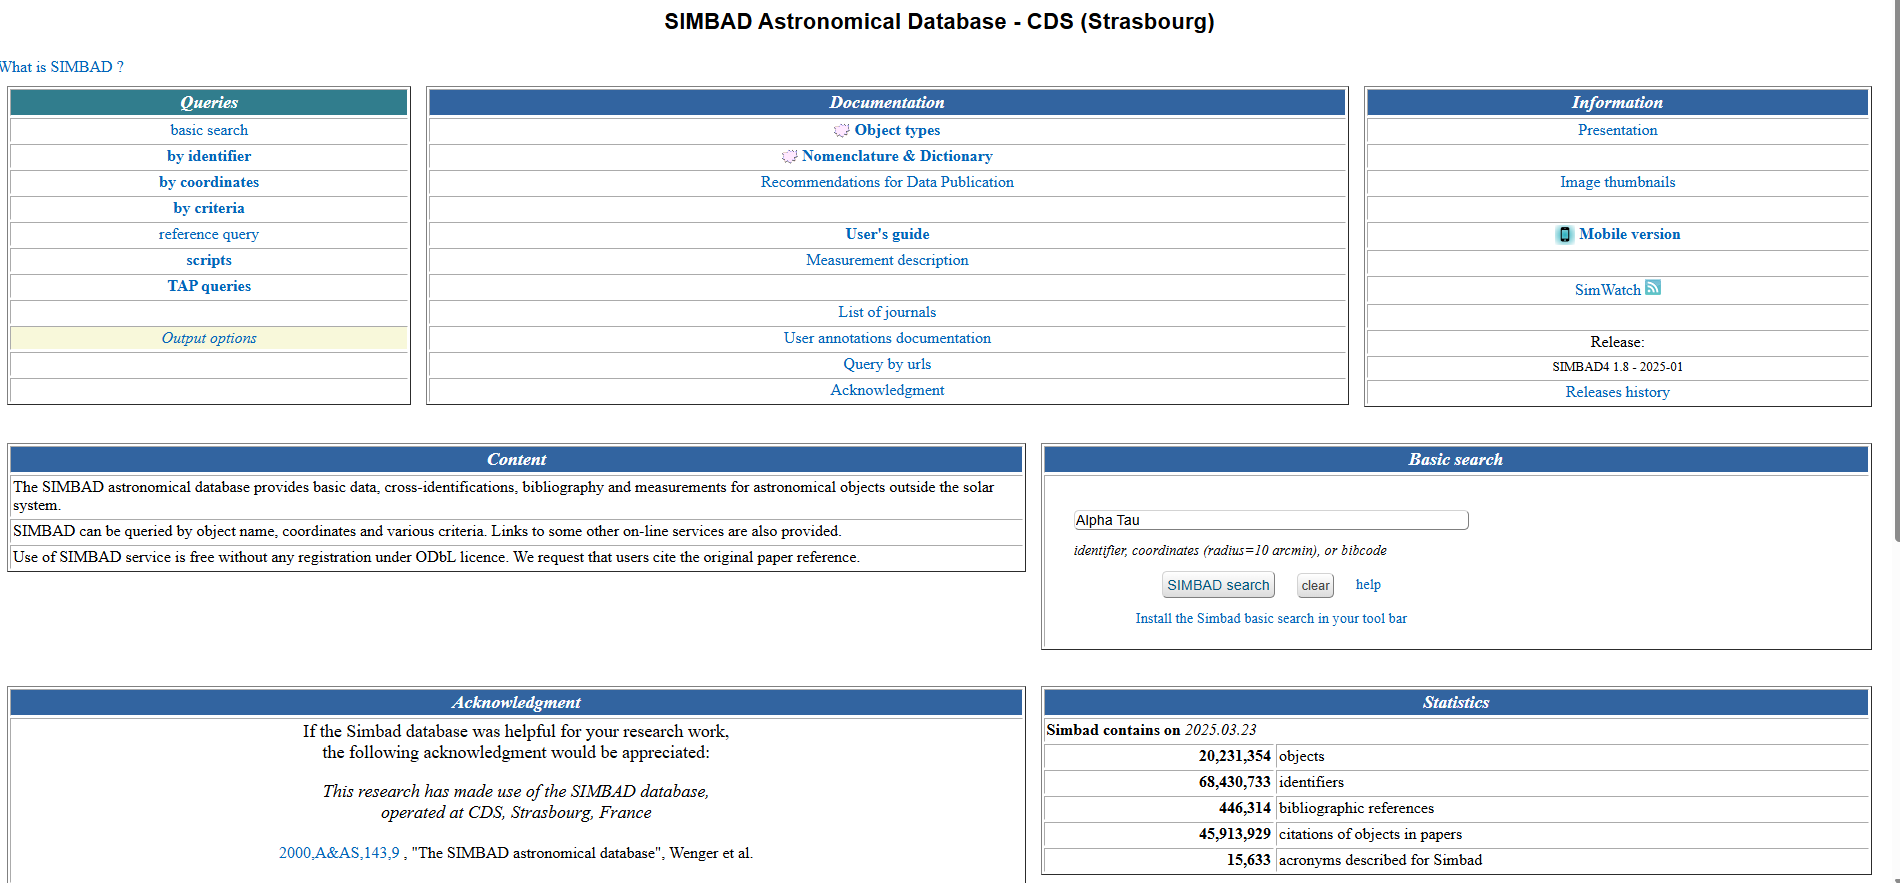
\includegraphics[width=0.5\textwidth]{SINBAD1.png}
    \caption{SINBAD Database homepage with search bar filled out.} 
    \label{fig:Alderbaran}
\end{figure}

You may try searching for Alderbaran, however many databases use the name Alpha Tauri(alf Tau). You'll be met with a basic data page and a list of previous measurements and observations. The data page will include the spectral type, mass, and temperature of the star and even more!

\section{Preparing Your Manuscript}
\end{document}